\documentclass[11pt]{article}

\usepackage[margin=1in]{geometry}
\usepackage[utf8]{inputenc}
\usepackage[T1]{fontenc}
\usepackage{amsmath,amssymb}
\usepackage{booktabs}
\usepackage{multirow}
\usepackage{graphicx}
\usepackage{xcolor}
\usepackage{tikz}
\usetikzlibrary{arrows.meta,positioning}
\usepackage[colorlinks=true,linkcolor=blue!60!black,citecolor=blue!60!black,urlcolor=blue!60!black]{hyperref}
\usepackage[round]{natbib}

\newcommand{\todo}[1]{\textcolor{red!70!black}{[TODO: #1]}}
\newcommand{\corpusA}{\textsc{Corpus~A}}
\newcommand{\corpusB}{\textsc{Corpus~B}}
\newcommand{\benchname}{Scientific Question Backtesting}
\newcommand{\labelfmt}[1]{\texttt{#1}}

\title{Historical Backtesting for Scientific Question Discovery:\\
A Protocol and Astronomy Pilot\\[0.6em]
\large Evaluating AI-Generated Scientific Questions Against Future
Scientific Progress}

\author{%
  \todo{author list}\\
  \todo{affiliations}
}
\date{\today}

\begin{document}

\maketitle

\begin{abstract}
Systems that generate scientific research questions are currently
evaluated by expert scores, LLM-as-judge ratings, or curated case
studies---all subjective, none falsifiable. We propose a different
standard: \emph{a scientific question is valuable if future science
actually invests in answering it}. We formalize \textbf{historical
backtesting} as an evaluation protocol for scientific question
discovery: a system generates questions from a corpus frozen at a
historical cutoff, the questions are frozen before any access to later
literature, and a temporally isolated future corpus determines---via
fixed retrieval, a citation-constrained judge, and human
adjudication---whether each question was subsequently answered,
partially addressed, independently posed, or ignored, and whether its
underlying premise was supported or refuted. The protocol is
model-agnostic: any system that emits frozen questions can be scored,
and all metrics are defined independently of how questions are produced.
We release a reproducible astronomy benchmark instance
(cutoff 2020-12-31): a 2{,}512-paper past corpus, a temporally isolated
1{,}891-paper future corpus (2021--2026), frozen questions, retrieval
records, adjudicated outcome labels, and one-command metric computation,
plus a submission interface and four reference baselines. In an initial
set of ten questions generated by an evidence-graph system from
pre-cutoff literature only, all ten were substantively engaged by later
literature: two were answered, seven partially addressed, one
independently posed and still open---and one question's underlying
premise (a strongly subsolar water abundance for HD~209458\,b) was
subsequently refuted by three independent analyses, the exact
convergence the question called for. We analyze failure modes and
threats to validity, and position this pilot as the initial instance of
a benchmark that any question-discovery system can run against.
\end{abstract}

\section{Introduction}
\label{sec:intro}

A growing family of systems claims to generate scientific research
questions, hypotheses, or ideas
\citep{lu2024aiscientist,wang2024scimon,baek2024researchagent}. How do we
know whether any of them is good at it? Today, essentially every
evaluation falls into one of three patterns: an \emph{expert score} (a
panel rates novelty and significance on a Likert scale), an \emph{LLM
score} (a language model rates the same properties), or a \emph{case
study} (a handful of generated ideas is narrated persuasively). All
three share the same defect: they are subjective. Expert panels disagree
with each other and with themselves \citep{si2024llmideas}; LLM judges
inherit the biases of their training distribution and can be steered by
phrasing; case studies are selected by the authors. None of these
evaluations can be \emph{wrong} in a way that data could demonstrate,
which is another way of saying none of them measures anything.

Science itself offers a harder criterion. Research questions are bets
about where inquiry should go next, and the scientific community
eventually settles those bets: it invests observing time, funds
follow-ups, writes papers that answer some questions, poses others
independently, and refutes the premises of a few. This suggests a simple
standard:

\begin{quote}
\emph{A scientific question is valuable if future science actually
invests in answering it.}
\end{quote}

The standard becomes an evaluation protocol the moment we rewind the
clock. Fix a historical cutoff. Give a system only the literature
available before the cutoff. Freeze the questions it generates. Then let
the literature published \emph{after} the cutoff---which the system
never saw---grade the bet: Was the question answered? Substantially
advanced? Independently posed by working scientists? Ignored? Was its
underlying premise confirmed, or refuted? We call this procedure
\textbf{historical backtesting}, by analogy with the evaluation of
trading strategies on held-out past data \citep{bailey2014backtest}, and
with recent forecasting benchmarks that score models against events
occurring after training \citep{zou2022autocast}.

\begin{figure}[t]
\centering
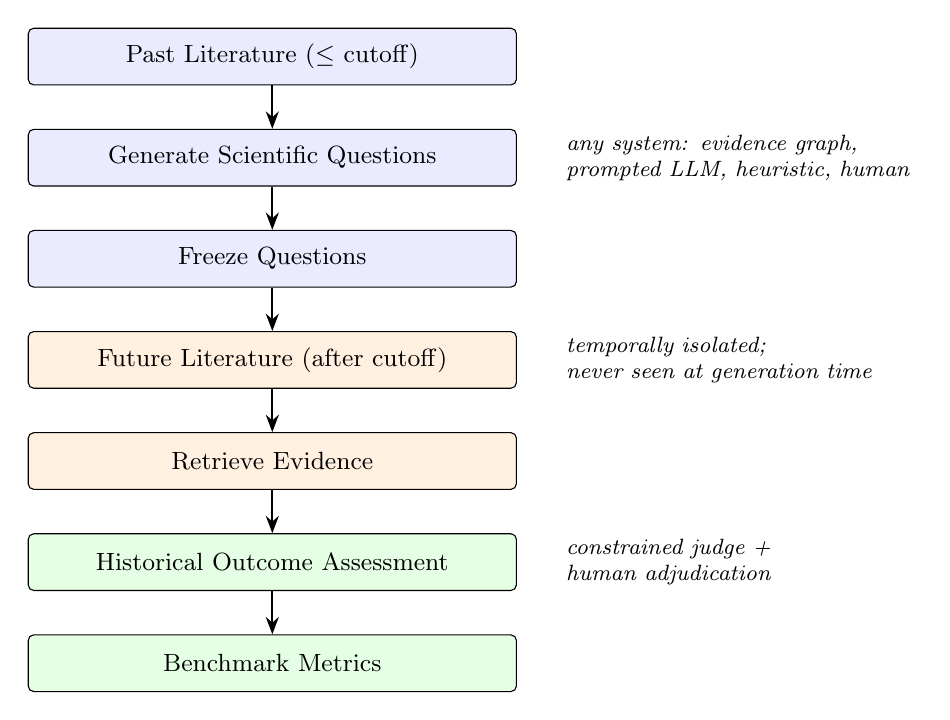
\begin{tikzpicture}[
    node distance=0.55cm,
    stage/.style={draw, rounded corners=2pt, minimum width=6.2cm,
                  minimum height=0.72cm, align=center, font=\small},
    past/.style={stage, fill=blue!8},
    future/.style={stage, fill=orange!12},
    eval/.style={stage, fill=green!10},
    arr/.style={-{Stealth[length=2.2mm]}, thick}]
  \node[past]   (p1) {Past Literature ($\leq$ cutoff)};
  \node[past,   below=of p1] (p2) {Generate Scientific Questions};
  \node[past,   below=of p2] (p3) {Freeze Questions};
  \node[future, below=of p3] (f1) {Future Literature (after cutoff)};
  \node[future, below=of f1] (f2) {Retrieve Evidence};
  \node[eval,   below=of f2] (e1) {Historical Outcome Assessment};
  \node[eval,   below=of e1] (e2) {Benchmark Metrics};
  \draw[arr] (p1) -- (p2);
  \draw[arr] (p2) -- (p3);
  \draw[arr] (p3) -- (f1);
  \draw[arr] (f1) -- (f2);
  \draw[arr] (f2) -- (e1);
  \draw[arr] (e1) -- (e2);
  \node[right=0.5cm of p2, font=\footnotesize\itshape, text width=4.4cm, align=left]
    {any system: evidence graph,\\ prompted LLM, heuristic, human};
  \node[right=0.5cm of f1, font=\footnotesize\itshape, text width=4.4cm, align=left]
    {temporally isolated;\\ never seen at generation time};
  \node[right=0.5cm of e1, font=\footnotesize\itshape, text width=4.4cm, align=left]
    {constrained judge +\\ human adjudication};
\end{tikzpicture}
\caption{The historical backtesting protocol. No question generator,
evidence graph, or particular LLM appears in the loop: the protocol
evaluates \emph{frozen question lists}, whatever produced them.}
\label{fig:protocol}
\end{figure}

Crucially, the protocol contains no question generator
(Figure~\ref{fig:protocol}). It takes a frozen list of questions as
input and returns outcome labels and metrics as output. Any
system---an evidence-graph pipeline, a prompted LLM, a citation
heuristic, a human scientist---can be evaluated under identical
conditions. This is what makes it a benchmark rather than a validation
appendix for one particular architecture.

\paragraph{Contributions.} We make three claims, in decreasing order of
strength:

\begin{enumerate}
  \item \textbf{Protocol (strong).} We formalize historical backtesting
    as an evaluation protocol for scientific question discovery:
    temporal isolation rules, a question-freezing requirement, fixed
    future-evidence retrieval, a two-dimensional outcome taxonomy that
    separates a question's fate (\labelfmt{answered},
    \labelfmt{partially\_addressed}, \labelfmt{posed\_but\_open},
    \labelfmt{not\_addressed}) from its premise's fate
    (\labelfmt{supported}, \labelfmt{refuted}, \labelfmt{weakened},
    \labelfmt{still\_plausible}, \labelfmt{not\_applicable}), and
    metrics defined over those labels (Sections~\ref{sec:protocol}
    and~\ref{sec:metrics}).
  \item \textbf{Benchmark instance (medium).} We release a reproducible
    astronomy instance with temporally isolated past and future corpora
    (2{,}512 and 1{,}891 papers; cutoff 2020-12-31), frozen questions,
    released retrieval records, adjudicated labels, one-command metric
    computation with CI-enforced reproducibility, a submission format,
    and four reference baselines (Sections~\ref{sec:dataset}
    and~\ref{sec:baselines}).
  \item \textbf{Empirical pilot (cautious).} In an initial set of ten
    questions generated from pre-cutoff evidence only, all ten were
    substantively engaged by the 2021--2026 literature, including one
    whose underlying premise was subsequently refuted by three
    independent analyses (Section~\ref{sec:results}). With $n=10$
    questions from one system in one domain, we do \emph{not} claim
    that AI can reliably identify the most valuable future scientific
    questions; we claim the protocol can tell us, eventually, whether
    it can.
\end{enumerate}

What we believe is ultimately most useful here is not any single
result but the change of category: scientific question quality moves
from a matter of taste (``this question seems interesting'') to a
measured, comparable quantity (``under historical backtesting, 100\% of
this system's questions were engaged by later literature; 10\% led to a
premise refutation''). Every artifact needed to run the protocol---data,
code, labels, and checks---is public, and Astronomy~v1 is offered as the
first instance of the benchmark, not as its definition.

\section{Related Work}
\label{sec:related}

\paragraph{Automated scientific discovery and question generation.}
Computational discovery has a long lineage, from rule-based rediscovery
of physical laws \citep{langley1987} through closed-loop robot
scientists \citep{king2009} to the Nobel Turing Challenge's call for
AI scientists \citep{kitano2021}. Recent LLM-based systems generate
research ideas, hypotheses, or full papers: literature-based generation
\citep{wang2024scimon}, agentic idea refinement
\citep{baek2024researchagent}, and end-to-end automated research
\citep{lu2024aiscientist}. Literature-based discovery pioneered the
underlying intuition that recombining published evidence can anticipate
findings later verified empirically \citep{swanson1986}. Our work is
orthogonal to all of these: we do not propose a better generator; we
propose the missing evaluation.

\paragraph{Evaluating generated ideas.}
Existing evaluations are dominated by human preference and LLM scoring.
\citet{si2024llmideas} ran a large expert study comparing human and LLM
research ideas on rated novelty and excitement---the most rigorous
instance of the expert-score paradigm, and still a measurement of
\emph{opinion at generation time} rather than of what the ideas turned
out to be worth. LLM-as-judge scoring inherits known biases (position,
verbosity, self-preference) and, for questions about the future,
cannot be validated against ground truth at all. Historical backtesting
replaces both with an outcome variable that exists independently of any
rater: the subsequent behavior of the scientific community.

\paragraph{Backtesting and forecasting benchmarks.}
Scoring a strategy on held-out history is standard in quantitative
finance, along with well-documented failure modes---overfitting to the
backtest itself \citep{bailey2014backtest}---that motivate our
freezing and no-overwrite rules. Forecasting benchmarks score models on
events that resolve after training \citep{zou2022autocast}; retrodictive
evaluation with temporal holdouts is likewise used to test whether
models anticipate later discoveries \citep{swanson1986,king2009}.
We transplant this design to a harder target: not whether a stated
event occurs, but whether an open-ended research question earns the
community's future investment. Code benchmarks such as SWE-bench
\citep{jimenez2024swebench} demonstrated how a well-specified task
format plus frozen data can reorganize a research area around
measurable progress; we aim the same mechanism at question discovery.

\paragraph{Data contamination.}
Temporal splits are increasingly used to control LLM memorization in
evaluation. Our protocol controls the \emph{retrieval} channel
completely (corpus manifests, isolation rules, CI checks) and treats the
\emph{weights} channel---models whose training data postdates the
cutoff---as a declared, audited threat rather than a solved problem
(Section~\ref{sec:threats}).

\section{The Historical Backtesting Protocol}
\label{sec:protocol}

The protocol evaluates a set of frozen questions $Q = \{q_1,\dots,q_n\}$
against a future corpus. It has six steps; each is fully specified so
that two groups running the same instance obtain the same measurement.

\subsection{Step 1: Choose a cutoff}
A historical date $T$ (Astronomy~v1: 2020-12-31) splits the literature
into a \emph{past corpus} \corpusA{} (everything available up to $T$)
and a \emph{future window} realized as an isolated corpus \corpusB{}
(strictly after $T$). The cutoff must be far enough in the past for the
community to have had time to act---we recommend $\geq 4$ years---and
recent enough that the past corpus reflects a modern research frontier.

\subsection{Step 2: Generate questions}
Any method may generate questions: an evidence-graph pipeline, a
prompted LLM, a heuristic over citation statistics, a human expert. The
only requirements are (i) the generator consumes \emph{only} \corpusA{}
evidence, and (ii) every question records the pre-cutoff evidence it is
grounded in (\texttt{source\_evidence\_ids}). A submission whose source
evidence postdates $T$ is invalid, mechanically
(\texttt{scripts/validate\_cutoff.py}).

\subsection{Step 3: Freeze}
Questions are serialized---identifier, text, cutoff, generating system,
source evidence, system-assigned rank---with \texttt{frozen:\,true}
\emph{before any access to post-cutoff literature}, and are never edited
afterwards. Freezing is the protocol's load-bearing rule: without it,
question text drifts toward what the evaluator has meanwhile learned the
future contains, and the backtest silently becomes a description of the
future rather than a prediction of it \citep{bailey2014backtest}. In the
released implementation frozen files are append-only and guarded by CI;
editing a released question mints a new versioned instance rather than
overwriting the old one.

\subsection{Step 4: Define the future window}
\corpusB{} is collected under its own frozen manifest (query set, date
window, deduplication rules) and stored separately from \corpusA{};
records from \corpusB{} must never enter the generation pipeline. The
Astronomy~v1 window is 2021--2026. Bounding the window matters for
comparability: ``eventually engaged'' is not a fixed target, but
``engaged within $k$ years'' is.

\subsection{Step 5: Retrieve future evidence}
For each frozen question, the question text and every \corpusB{}
document (title + abstract) are embedded
(\texttt{text-embedding-3-small}); the top-$k$ documents by cosine
similarity ($k=8$) become the candidate evidence. Retrieval is
deliberately fixed and deliberately simple: systems are compared on
their \emph{questions}, not their retrievers, and reviewers can inspect
exactly which documents the judge saw because retrieval records are part
of the release.

\subsection{Step 6: Assess outcomes}
\label{sec:protocol:outcomes}

A judge reads the question and its retrieved candidates and assigns two
\emph{independent} labels (Table~\ref{tab:taxonomy}): the fate of the
question and the fate of its premise.

\begin{table}[t]
  \centering
  \small
  \caption{Outcome taxonomy v1.0. The two dimensions are labeled
  independently.}
  \label{tab:taxonomy}
  \begin{tabular}{@{}llp{8.2cm}@{}}
    \toprule
    Dimension & Label & Meaning \\
    \midrule
    \multirow{4}{*}{\texttt{outcome}}
      & \labelfmt{answered} & Future evidence substantially answers the question (including by refuting its premise) \\
      & \labelfmt{partially\_addressed} & Important, directly relevant progress; core question unresolved \\
      & \labelfmt{posed\_but\_open} & The community independently poses essentially the same question without resolving it \\
      & \labelfmt{not\_addressed} & No meaningful follow-up in the future corpus \\
    \midrule
    \multirow{5}{*}{\texttt{premise\_status}}
      & \labelfmt{supported} & Future evidence confirms the underlying premise \\
      & \labelfmt{refuted} & Future evidence falsifies the underlying premise \\
      & \labelfmt{weakened} & Substantial doubt cast without falsification \\
      & \labelfmt{still\_plausible} & The premise was not directly tested after the cutoff \\
      & \labelfmt{not\_applicable} & The question rests on no contestable premise \\
    \bottomrule
  \end{tabular}
\end{table}

Two design decisions deserve emphasis. First, the dimensions are
separated because the single most informative outcome a backtest can
surface---\emph{the community answered this question by refuting its
premise}---is inexpressible in a flat label set: it is simultaneously a
resolution (\labelfmt{answered}) and a falsification
(\labelfmt{refuted}). Our pilot's headline case
(Section~\ref{sec:results:case}) is exactly of this type. Second,
premise refutation is scored as a \emph{success} of the question, not a
failure: a question that provokes the community into overturning one of
its own published conclusions has done the most a question can do.

The judge operates under hard constraints enforced outside the model:
it may cite only bibcodes from the retrieved candidates (violations are
errors, never silently dropped); topical similarity is explicitly
insufficient---the cited paper must bear on the question's actual test
or premise; unknown labels fall back to the most conservative value and
are flagged. Labels then occupy one of two declared tiers.
\emph{Adjudicated} labels have passed human review under written
guidelines (citation validity, the engagement bar, the outcome/premise
split), with the adjudication log released; the headline labels of a
released instance are required to be of this tier (Astronomy~v1's are).
\emph{Judge-only} labels have not, are marked as such wherever
reported, and are the tier at which this paper's large-$n$ comparative
studies run (Sections~\ref{sec:scaled}--\ref{sec:foresight}). The
tier is part of every result's provenance; conflating them is a
protocol violation.

\subsection{Submissions}
A system is evaluated by submitting a directory containing
\texttt{questions.jsonl} (the frozen questions) and
\texttt{metadata.json} (system description, including a mandatory
declaration of any LLM components and their versions, for contamination
auditing). The benchmark pipeline---isolation checks, retrieval,
judging, adjudication where the tier requires it, metrics,
report---is identical for every
submission; the system whose questions we evaluate in
Section~\ref{sec:results} interacts with the benchmark only through
this interface.

\section{Benchmark Metrics}
\label{sec:metrics}

Let $Q$ be the $n$ frozen questions of a submission, with outcome labels
$o(q)$ and premise labels $p(q)$ as in Table~\ref{tab:taxonomy}, and let
$E(q)$ be the set of independent post-cutoff papers cited as supporting
evidence for $q$'s label. All rates are over $n$, so the four outcome
rates sum to one.

\begin{table}[t]
  \centering
  \small
  \caption{Benchmark metrics v1.0. All are computed by
  \texttt{benchmark/metrics.py} from the released annotation records.}
  \label{tab:metrics}
  \begin{tabular}{@{}lp{9.6cm}@{}}
    \toprule
    Metric & Definition \\
    \midrule
    Coverage (future attention rate) &
      $\frac{1}{n}\,|\{q : o(q) \neq \labelfmt{not\_addressed}\}|$ ---
      did future science engage the question at all? \\
    Answer rate &
      $\frac{1}{n}\,|\{q : o(q) = \labelfmt{answered}\}|$ \\
    Partial rate &
      $\frac{1}{n}\,|\{q : o(q) = \labelfmt{partially\_addressed}\}|$ \\
    Open rate &
      $\frac{1}{n}\,|\{q : o(q) = \labelfmt{posed\_but\_open}\}|$ ---
      the community independently recognized the question \\
    Premise refutation rate &
      $\frac{1}{n}\,|\{q : p(q) = \labelfmt{refuted}\}|$ ---
      questions that led to an established conclusion being overturned \\
    Evidence strength &
      mean $|E(q)|$ over engaged questions, and the multi-source rate
      $\frac{1}{n}\,|\{q : |E(q)| \geq 2\}|$ --- is the label supported
      by multiple independent papers? \\
    Lead time &
      years between question submission and the first time the community
      \emph{independently poses} the same question \\
    Community attention &
      volume of future investment engaging the question: papers,
      citations, review mentions, and major observing programs (e.g.\
      JWST/HST proposals) \\
    \bottomrule
  \end{tabular}
\end{table}

\paragraph{Coverage vs.\ answer rate.} Coverage asks whether the
question pointed anywhere the community went at all; the answer/partial/
open decomposition asks what happened when it got there. A system can
maximize coverage with fashionable-topic questions, which is why
coverage is never reported alone (Section~\ref{sec:threats} discusses
the popularity confound).

\paragraph{Premise refutation rate.} This is the metric we most want the
field to adopt. Questions that trigger refutations are the rarest and
arguably most valuable output of question discovery---they mark places
where the literature's accepted conclusions were wrong and where a
well-aimed question preceded the correction. Under the two-dimensional
taxonomy the refutation is recorded without erasing the fact that the
question was thereby \emph{answered}.

\paragraph{Lead time.} If a system poses a question at the cutoff and
the community first independently poses it in year $T{+}\ell$, the
system led the field by $\ell$ years; averaged over questions this
yields a comparable earliness score. Measuring $\ell$ requires
identifying \emph{community first-posed dates}, which demands careful
review-literature annotation we do not yet have. Astronomy~v1 therefore
reports \texttt{mean\_lead\_time\_years:\,null} rather than a number we
cannot defend; the released records do include a weaker, well-defined
lower bound---\emph{first-engagement lag}, the years from cutoff to the
earliest judge-cited supporting paper (pilot mean 2.9, range 1--5)---
which should not be confused with lead time.

\paragraph{Community attention.} Beyond binary engagement, the volume of
future investment (paper counts, citations to engaging papers, review
mentions, dedicated observing programs) reflects how much the community
cared. v1 records the ingredients (supporting bibcodes, their venues and
years) and reports evidence strength; a calibrated attention index is
future work, and Section~\ref{sec:threats} explains why raw attention
must never be the headline metric.

\paragraph{Reporting requirements.} A benchmark report must state: the
instance and protocol versions, $n$, all outcome and premise rates, the
evidence-strength pair, and either lead time or an explicit null. The
released implementation produces exactly this
(\texttt{results/astronomy\_v1/metrics.json}) with one command, and CI
fails if the committed numbers do not reproduce from the raw
annotations.

\section{The Astronomy v1 Instance}
\label{sec:dataset}

Astronomy~v1 instantiates the protocol in exoplanet atmospheres---a
domain chosen because it uniquely combines a fast-moving literature,
structured catalogs, and space-telescope archives, and because the
2021--2026 window contains a natural experiment: JWST began delivering
data mid-window, resolving questions that were unanswerable at the
cutoff. Table~\ref{tab:corpus} summarizes the instance.

\begin{table}[t]
  \centering
  \small
  \caption{Astronomy v1 at a glance. Corpus manifests, frozen questions,
  retrieval records, and adjudicated labels are all released.}
  \label{tab:corpus}
  \begin{tabular}{@{}ll@{}}
    \toprule
    Historical cutoff & 2020-12-31 \\
    Domain scope & atmospheric composition in transmission spectra;
                   cloud/haze degeneracies; instrument systematics \\
    \midrule
    \corpusA{} (past) & 2{,}512 deduplicated papers, 2015--2020 (NASA ADS;
                        500-paper full-text core) \\
    \corpusB{} (future) & 1{,}891 unique papers, 2021--2026, temporally
                          isolated \\
    Questions & 10, frozen, ranked, with pre-cutoff source evidence \\
    Retrieval & \texttt{text-embedding-3-small}, cosine, top-8; records released \\
    Judge & \texttt{gpt-4.1}, temperature 0, citation-constrained;
            human-adjudicated \\
    \bottomrule
  \end{tabular}
\end{table}

\paragraph{Corpora.} Both corpora are defined by frozen manifests---ADS
query sets, date windows, deduplication and filtering rules
(records without abstracts are dropped)---rather than by bulk data
dumps: the manifests are committed, and a script rebuilds either corpus
from its manifest via the ADS API. \corpusB{}'s manifest adds targeted
follow-up queries for the questions' objects (HD~189733, HD~209458,
WASP-12, WASP-121, TRAPPIST-1) so that engagement is measured against
the relevant future literature rather than against whatever a generic
query happens to return.

\paragraph{Leakage controls.} Temporal isolation is enforced
mechanically, not editorially: (1) nothing dated after the cutoff may
enter \corpusA{}, including catalog rows updated post-cutoff; (2) every
question's source evidence must predate the cutoff; (3) every retrieved
document must postdate it; (4) the judge may cite only retrieved
candidates; (5) question/retrieval/annotation records must align
one-to-one; (6) \corpusB{}'s window must start strictly after the
cutoff. All six checks run in continuous integration on every change to
the released data, together with a check that the released
\texttt{metrics.json} reproduces bit-identically from the raw
annotations.

\paragraph{Questions.} The ten frozen questions were generated by an
evidence-graph system \citep{paper1} from \corpusA{} only: claims with
provenance are extracted from the full-text core, cross-paper tensions
are detected and typed (observational tensions, methodological
challenges, single-dataset conclusions, independent qualifications), and
surviving signals are refined into ranked, falsifiable questions. For
the benchmark, that system is submission
\texttt{evidence\_graph\_v1}---evaluated through the same interface as
any future submission. Each released record carries the question text,
system rank, signal type, target objects, and pre-cutoff source
bibcodes; a curation log documenting human edits made \emph{before}
freezing (including a near-duplicate merge and presupposition fixes,
Section~\ref{sec:errors}) is released for audit.

\paragraph{What is released.} Frozen questions; corpus manifests; per-
question retrieval records (model, window, top-$k$, judge-cited
documents, top-1 similarity; full ranked lists with scores are scheduled
for v1.1); adjudicated outcome annotations with rationales and
supporting bibcodes; the adjudication log; computed metrics and
per-question results; four frozen baseline submissions with their full
retrieval records (per-document scores included), judge annotations,
and reports (Section~\ref{sec:baselines}); the scaled v1L instance
(manifests, configs, 424 frozen baseline questions, retrieval records
with per-document scores, judge annotations, per-system reports, and
the statistical comparison script of Section~\ref{sec:scaled}); the
tension-pair generators, the four-cutoff stress-test corpora manifests,
all 798 stress-test judgments, and the deterministic specificity rubric
of Section~\ref{sec:foresight}; and the complete pipeline code with
tests. The
data format is deliberately plain (JSONL + JSON manifests) so that other
groups can mint new instances---different domain, different cutoff---by
writing two manifests and one config file.

\section{Baselines}
\label{sec:baselines}

A benchmark that only ever scored one system would be a validation
appendix. Astronomy~v1 ships four reference baselines, chosen to
bracket the interesting comparisons; each consumes only \corpusA{}
records, freezes its output before any future-corpus access, and is
evaluated through the identical pipeline.

\begin{description}
  \item[B1: Random claims.] Sample random pre-cutoff papers and template
    their headline result into a robustness question. The floor: any
    system must beat chance-directed attention.
  \item[B2: Direct LLM.] Give an LLM a sample of pre-cutoff abstracts
    and ask for the most valuable open questions. The ``why not just ask
    GPT?'' comparison. Because a modern LLM's weights postdate the
    cutoff, this baseline is also a contamination probe: performance
    that vanishes for post-training-cutoff instances indicates
    memorized hindsight rather than generation ability
    (Section~\ref{sec:threats}).
  \item[B3: Review future work.] Extract explicitly posed open questions
    from pre-cutoff review papers. The strongest natural reference: a
    discovery system is interesting only if it adds value over questions
    the community had already written down. Note this baseline should
    score highly on coverage \emph{by construction}---these questions
    are known community priorities---so the discriminating metrics are
    premise refutation and lead time, where a copied question can never
    lead the field.
  \item[B4: Citation leaders.] Template follow-up questions from the
    most-cited pre-cutoff papers. Tests whether chasing prominence
    matches structured evidence analysis.
\end{description}

\begin{table}[t]
  \centering
  \small
  \caption{Astronomy v1 leaderboard. The pilot release scores one
  submission; baseline rows will be populated from the released harness
  (\texttt{baselines/}), and external systems can submit via the
  interface in Section~\ref{sec:protocol}. Lead time is reported as null
  until community first-posed dates are annotated
  (Section~\ref{sec:metrics}).}
  \label{tab:leaderboard}
  \begin{tabular}{@{}lccccc@{}}
    \toprule
    System & $n$ & Coverage & Answered & Premise refuted & Lead time \\
    \midrule
    \texttt{evidence\_graph\_v1} \citep{paper1} & 10 & 100\% & 20\% & 10\% & --- \\
    B1 random claims        & --- & --- & --- & --- & --- \\
    B2 direct LLM           & --- & --- & --- & --- & --- \\
    B3 review future work   & --- & --- & --- & --- & --- \\
    B4 citation leaders     & --- & --- & --- & --- & --- \\
    \bottomrule
  \end{tabular}
\end{table}

The pilot release implements the four baselines as runnable submission
generators but reports scores only for \texttt{evidence\_graph\_v1}
(Table~\ref{tab:leaderboard}): baseline outcome labels require the same
retrieval--judging--adjudication budget as any submission, and we
prefer an honest partially populated leaderboard over rushed labels.
Populating the baseline rows is the release's first roadmap item, and
the leaderboard file (\texttt{results/leaderboard.json}) is designed for
external submissions to append to.

\section{Pilot Results: Historical Validation}
\label{sec:results}

We ran the full protocol on the ten frozen
\texttt{evidence\_graph\_v1} questions. Headline numbers: every
question was substantively engaged by the 2021--2026 literature
(coverage 100\%); two were answered, seven partially addressed, one
independently posed and still open; one premise was refuted. Evidence
strength: 2.4 supporting papers per question on average, with 60\% of
labels supported by $\geq 2$ independent papers. The earliest
judge-cited engagement came 1--5 years after the cutoff (mean 2.9).
Table~\ref{tab:perq} gives the per-question picture.

\begin{table}[t]
  \centering
  \small
  \caption{Per-question outcomes for \texttt{evidence\_graph\_v1} on
  Astronomy v1 (system rank order; $|E|$ = independent supporting
  papers; year = earliest cited engagement).}
  \label{tab:perq}
  \begin{tabular}{@{}clllcc@{}}
    \toprule
    Rank & ID & Outcome & Premise & $|E|$ & Year \\
    \midrule
    1  & q\_002 & \labelfmt{posed\_but\_open}      & \labelfmt{still\_plausible} & 1 & 2022 \\
    2  & q\_001 & \labelfmt{partially\_addressed}  & \labelfmt{supported}        & 3 & 2021 \\
    3  & q\_004 & \labelfmt{partially\_addressed}  & \labelfmt{supported}        & 1 & 2021 \\
    4  & q\_008 & \labelfmt{answered}              & \labelfmt{refuted}          & 3 & 2025 \\
    5  & q\_007 & \labelfmt{partially\_addressed}  & \labelfmt{still\_plausible} & 3 & 2024 \\
    6  & q\_010 & \labelfmt{partially\_addressed}  & \labelfmt{still\_plausible} & 1 & 2022 \\
    7  & q\_005 & \labelfmt{answered}              & \labelfmt{supported}        & 2 & 2024 \\
    8  & q\_009 & \labelfmt{partially\_addressed}  & \labelfmt{supported}        & 5 & 2021 \\
    9  & q\_006 & \labelfmt{partially\_addressed}  & \labelfmt{still\_plausible} & 1 & 2025 \\
    10 & q\_011 & \labelfmt{partially\_addressed}  & \labelfmt{still\_plausible} & 4 & 2024 \\
    \bottomrule
  \end{tabular}
\end{table}

\subsection{Case study: a premise refuted (q\_008, HD 209458 b)}
\label{sec:results:case}

From pre-2021 evidence, the system flagged a single-dataset conclusion:
the influential retrieval of a \emph{strongly subsolar} water abundance
at the terminator of HD~209458\,b \citep{macdonald2017}. The frozen
question asked, in 2020 terms:

\begin{quote}\itshape
Is the strongly subsolar terminator water abundance retrieved for
HD~209458\,b a property of the atmosphere or an artifact of retrieval
assumptions, as tested by comparing independent retrieval frameworks on
the same and on independent datasets?
\end{quote}

The 2021--2026 literature then performed exactly the test the question
specified (Figure~\ref{fig:case}): a reanalysis of HST and JWST spectra
with improved systematics treatment and Bayesian model averaging, an
independent retrieval framework demonstrating that free-vs-equilibrium
chemistry assumptions span the subsolar-to-solar range, and ground-based
high-resolution spectroscopy constraining the abundance independently of
space-based data. All three converge: the terminator water abundance is
consistent with solar, and the strongly subsolar value was an artifact
of earlier retrieval assumptions and data systematics. Under the
taxonomy this is \labelfmt{answered} + \labelfmt{refuted}: the question
was resolved \emph{by} the community overturning the premise the
question challenged---an outcome that no expert score assigned in 2020
could have certified, and precisely what backtesting exists to detect.

\begin{figure}[t]
\centering
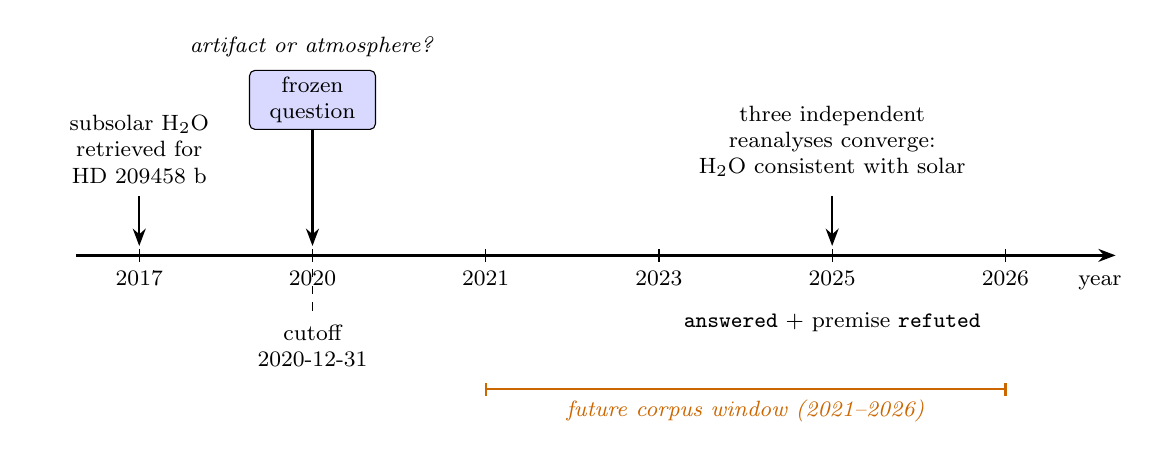
\begin{tikzpicture}[
    font=\small,
    evt/.style={align=center, font=\footnotesize},
    arr/.style={-{Stealth[length=2.2mm]}, thick}]

  \draw[arr] (0,0) -- (13.2,0);
  \node[font=\footnotesize] at (13.0,-0.35) {year};
  \foreach \x/\y in {0.8/2017, 3.0/2020, 5.2/2021, 7.4/2023, 9.6/2025, 11.8/2026}
    \draw (\x,0.08) -- (\x,-0.08) node[below, font=\footnotesize] {\y};

  \node[evt, text width=2.6cm] at (0.8,1.35)
    {subsolar H$_2$O\\ retrieved for\\ HD 209458 b};
  \draw[arr] (0.8,0.75) -- (0.8,0.12);

  \draw[fill=blue!15, rounded corners=2pt] (2.2,1.6) rectangle (3.8,2.35);
  \node[evt] at (3.0,1.975) {frozen\\ question};
  \draw[arr] (3.0,1.6) -- (3.0,0.12);
  \node[evt] at (3.0,2.65) {\emph{artifact or atmosphere?}};

  \draw[dashed] (3.0,-0.7) -- (3.0,1.4);
  \node[evt] at (3.0,-1.15) {cutoff\\ 2020-12-31};

  \node[evt, text width=3.4cm] at (9.6,1.45)
    {three independent\\ reanalyses converge:\\ H$_2$O consistent with solar};
  \draw[arr] (9.6,0.75) -- (9.6,0.12);
  \node[evt, text width=3.9cm] at (9.6,-0.85)
    {\labelfmt{answered} + premise \labelfmt{refuted}};

  \draw[thick, orange!80!black] (5.2,-1.7) -- (11.8,-1.7)
    node[midway, below, font=\footnotesize\itshape]
    {future corpus window (2021--2026)};
  \draw[thick, orange!80!black] (5.2,-1.78) -- (5.2,-1.62);
  \draw[thick, orange!80!black] (11.8,-1.78) -- (11.8,-1.62);
\end{tikzpicture}
\caption{Timeline of q\_008. The question was frozen from pre-2021
evidence; by 2025 three independent analyses had performed the test it
specified and refuted its premise---the strongly subsolar water
abundance was a retrieval artifact.}
\label{fig:case}
\end{figure}

\subsection{Secondary observations}

\paragraph{The top-ranked question is independently posed and open.}
The system's rank-1 question (q\_002: how terminator heterogeneity
biases the WASP-12\,b water abundance and C/O ratio) tracks a
methodological concern the community has since engaged in general form
--- inhomogeneous-terminator biases in retrievals --- without resolving
it for WASP-12\,b specifically: \labelfmt{posed\_but\_open}. A question
the field poses but has not answered is a live research target; that the
system's top pick lands there is the behavior a ranking is supposed to
produce, though $n=1$ at rank 1 proves nothing by itself.

\paragraph{An answered null result.} q\_005 asked whether HST
transmission data independently support NH$_3$ or HCN in HD~209458\,b
--- a molecular-detection claim from the same single-dataset analysis as
q\_008 \citep{macdonald2017}. By 2024--2025, high-resolution
spectroscopy had placed stringent upper limits on both species:
\labelfmt{answered}, premise \labelfmt{supported} (the data indeed do
not independently support the detection). Backtesting counts a
cleanly resolved null exactly as it counts a positive.

\paragraph{Instrument-gated engagement.} q\_011 (whether JWST validated
pre-launch predictions of TRAPPIST-1 CO$_2$ detectability,
\citealp{lustigyaeger2019}) could not have been engaged before JWST flew;
its first cited engagement is 2024 and stellar contamination has so far
prevented a definitive test. Engagement timing is partly an instrument
schedule, not purely a question-quality signal---a confound
Section~\ref{sec:threats} treats explicitly.

\paragraph{What these ten questions do not show.} With ten questions
from one system in one domain, rates carry wide intervals (the exact
95\% Clopper--Pearson interval for 10/10 coverage is $[0.69, 1.0]$),
the baseline rows are judge-only rather than adjudicated
(Section~\ref{sec:baselines}), and the generating system's LLM
components postdate the cutoff (Section~\ref{sec:threats}). The pilot
demonstrates that the protocol runs end-to-end, yields auditable,
reproducible labels, and prices its baselines; it does not establish
that any system reliably anticipates future science.

\section{Error Analysis}
\label{sec:errors}

The released curation log records every human intervention made before
freezing; the failure modes below are taken from it and from the
adjudication log, and each motivates a benchmark rule.

\paragraph{Question duplication.} The generator produced near-duplicate
questions (q\_002/q\_003) from the same claim pair, differing mainly in
emphasis; they were merged during curation into one question with two
sub-questions. Left unmerged, duplicates would double-count a single
insight in every rate. Rule: submissions are screened for
near-duplicates, and instances should report a deduplication note; a
mechanical similarity screen is a v1.1 roadmap item.

\paragraph{Leading questions (presupposition).} Several generated
questions presupposed their own answer. q\_001 originally asserted that
vertical wind shear \emph{exists} rather than asking what causes the
wind-speed discrepancy; q\_008 originally presupposed the subsolar water
abundance rather than framing artifact-vs-atmosphere attribution. A
question that presupposes its answer cannot be cleanly refuted---and
q\_008's later refutation was only expressible because curation reframed
it as attribution. Rule: the quality gate flags presupposing phrasings
before freezing; the reframing is logged.

\paragraph{Self-contradictory quantifiers.} q\_003's original phrasing
asked whether a detection was ``robust to biases exceeding an order of
magnitude''---a bias that large \emph{is} non-robustness. Templated
quantifier language can silently produce unanswerable questions; the
clarity gate exists for this.

\paragraph{Conflated statistical and physical framing.} q\_010
originally asked what ``temperature and pressure conditions'' produce a
5.4$\sigma$ water detection, conflating atmospheric state with the
detection pipeline (significance depends on noise model, priors, null
hypothesis---not on the atmosphere). It was reframed as a sensitivity
analysis; its score on the generator's internal 0--10 clarity gate
(6.0) was the lowest of the set, and
its outcome (\labelfmt{partially\_addressed} on one supporting paper)
remains among the weakest-evidenced labels.

\paragraph{Premise bias in generation.} The generator inherits the
premises of the papers it reads: single-dataset conclusions taken at
face value can produce questions that merely restate a claim rather
than test it. The tension-typing stage (which explicitly marks
\emph{single-dataset conclusion} as a signal type) partially controls
this---q\_008 and q\_005 are that control working---but the benchmark's
premise dimension is the systematic check: a healthy portfolio should
show a mix of \labelfmt{supported} and \labelfmt{refuted}, not uniform
support of its sources.

\paragraph{Retrieval near-misses.} Judged evidence for q\_007
(HD~189733\,b / HAT-P-11\,b patchy clouds) leans partly on a
three-retrieval-framework study of HAT-P-\emph{18}\,b---directly
relevant methodologically, but not the named targets. The adjudication
log records the engagement-bar judgment; releasing full top-8 lists
(v1.1) will let others re-litigate such calls, which is the point of
releasing them.

\section{Threats to Validity}
\label{sec:threats}

Historical backtesting removes rater subjectivity; it does not remove
every confound. We enumerate the serious ones and what the protocol
does---and cannot do---about each.

\paragraph{Future inattention is not question badness.} A question can
be ignored because the enabling instrument never flew, the community's
funding shifted, or the subfield is small---not because the question was
poor. q\_011 was unanswerable before JWST delivered TRAPPIST-1 spectra;
had JWST slipped five years, an excellent question would have scored
\labelfmt{not\_addressed}. Mitigations: bounded windows make the
censoring explicit; \labelfmt{posed\_but\_open} separates
``recognized but unresolved'' from ``ignored''; instances should be
read as \emph{engagement within $k$ years given the era's instruments},
not as timeless value.

\paragraph{Future attention is not question goodness.} Symmetrically, a
question on a fashionable topic collects engagement for reasons other
than merit; coverage alone can be gamed by asking about whatever is
popular. Mitigations: coverage is never reported alone; premise
refutation and (future) lead time cannot be earned by fashion-chasing;
baseline B4 (citation leaders) exists precisely to price in prominence;
and the engagement bar requires the cited paper to bear on the
question's actual test, not its topic.

\paragraph{LLM training contamination.} The generating system and the
judge both use models whose training data postdates the cutoff. The
protocol seals the retrieval channel, not the weights channel: a model
may ``know'' the 2025 refutation while drafting a 2020-framed question.
This is the deepest threat to any backtest run with modern models.
Mitigations, none complete: source-evidence audit forces every question
to be grounded in cited pre-cutoff evidence; submission metadata must
declare all LLM components and versions; baseline B2 doubles as a
contamination probe---and registers one: its questions sit measurably
closer to the future literature's phrasing than any other system's
($s_1 = 0.732$, Table~\ref{tab:leaderboard}) while resolving nothing,
the signature of phrasing-level memorization without specific
foresight; and the decisive test is \emph{prospective}
instances---questions frozen today and scored in 2030 cannot be
contaminated. The protocol is explicitly designed so its instances
convert from retrospective to prospective by just letting time pass.

\paragraph{Judge and adjudicator reliability.} A single LLM judge,
even citation-constrained and human-adjudicated, is one reading of the
evidence; abstracts (not full texts) bound what it can see, and the
adjudicators are not blind to which system produced the questions.
Mitigations: labels ship with rationales and citations so any label is
independently checkable; disagreement is handled by written conservative
rules (prefer the weaker engagement); multi-judge agreement measurement
and blinded adjudication are roadmap items.

\paragraph{Retrieval as a bottleneck.} Top-8 abstract-embedding
retrieval can miss engaging papers (undercounting engagement) or
surface topically similar non-engagement (which the judge must reject).
Fixed retrieval is a deliberate trade: it makes comparisons across
systems fair and auditable at the cost of an engagement floor.
Sensitivity of labels to $k$ and to the retriever is measurable within
the released data schema and belongs in v1.1.

\paragraph{Small $n$, one domain, self-evaluation.} Ten questions per
system in one domain, evaluated by the group that built the leading
system, support no ranking claims---which is why the baseline rows are
labeled judge-only rather than adjudicated, the harness is public, and
the paper's empirical claim is deliberately modest
(Section~\ref{sec:intro}). At $n=10$ the leaderboard's answered-rate
differences (0--30\%) are within each other's confidence intervals; we
report them as priced reference points, not rankings. The protocol's
value grows with adversarial use by systems we did not build.

\paragraph{Curation hindsight.} Humans who edited questions before
freezing know the post-2020 literature. The curation log is released so
every edit is auditable (e.g.\ q\_008's reframing strengthened
falsifiability without smuggling in the answer), but retrospective
instances cannot fully exclude this channel; prospective ones can.

\section{Roadmap and Conclusion}
\label{sec:conclusion}

\paragraph{Roadmap.} The released instance is a floor, not a ceiling.
In order: (1) adjudicate the judge-only baseline rows
(Table~\ref{tab:leaderboard}) and accept external submissions;
(2) release full top-8 retrieval lists with per-document scores and a
near-duplicate screen (v1.1); (3) annotate community first-posed dates
in the review literature to activate lead time; (4) calibrate a
community-attention index (papers, citations, observing programs)
against the popularity confound; (5) mint instances in additional
domains and at additional cutoffs, including \emph{prospective}
instances---questions frozen now, scored when the future arrives---which
eliminate the contamination and hindsight channels entirely;
(6) measure judge robustness (multi-judge agreement, retrieval
sensitivity, blinded adjudication).

\paragraph{Conclusion.} We formalized historical backtesting as an
evaluation protocol for scientific question discovery, released a
reproducible astronomy instance with temporally isolated corpora and
fully auditable labels, and ran a ten-question pilot in which every
frozen question was substantively engaged by literature the generating
system never saw---including one whose premise the community
subsequently refuted, the exact convergence test the question had
specified. The individual numbers matter less than the category they
inhabit: for the first time, ``this system asks good scientific
questions'' is a claim with a denominator---falsifiable, comparable
across systems, and computable by anyone from frozen public data.
Question-asking has been argued to be a core capability on the path to
more general scientific intelligence \citep{kitano2021,paper1}; if that
is so, the field will need to measure it. This protocol, and this first
instance, are offered as the place to start---not as the definition of
the benchmark, but as its initial version, built to be superseded by
instances with more questions, more systems, more domains, and cutoffs
whose futures have not yet happened.


\bibliographystyle{plainnat}
\bibliography{references}

\end{document}
